\documentclass[titlepage,12pt,a4paper,times]{book}

\usepackage[utf8]{inputenc}
\usepackage[english]{babel}
\usepackage[T1]{fontenc}
\usepackage{makeidx}
\usepackage{xspace}
\usepackage{graphicx,color,times}
\usepackage{fancyhdr}
% \usepackage{pxfonts}
% \usepackage{times}
% \usepackage{mathptm}
% \usepackage{amssymb}
% \usepackage{amsfonts}
\usepackage{amsmath}
\usepackage{latexsym}
\usepackage[printonlyused]{acronym}
\usepackage{float}
\usepackage{listings}
\usepackage{tocbibind}
\usepackage{wrapfig}
\usepackage[square]{natbib}
\usepackage{hyperref}
% \usepackage{glossaries}
% \makeglossaries
\usepackage{etoolbox}
\usepackage[section]{placeins}
\usepackage{enumitem}

% reset acronyms every chapter
\preto\chapter{\acresetall}

\renewcommand{\ttdefault}{phv}

\pagestyle{fancy}
\renewcommand{\chaptermark}[1]{\markboth{#1}{}}
\renewcommand{\sectionmark}[1]{\markright{\thesection\ #1}}
\fancyhf{} \fancyhead[LE,RO]{\bfseries\thepage}
\fancyhead[LO]{\bfseries\rightmark}
\fancyhead[RE]{\bfseries\leftmark}
\renewcommand{\headrulewidth}{0.5pt}
\renewcommand{\footrulewidth}{0pt}
\addtolength{\headheight}{0.5pt}
\setlength{\marginparsep}{0cm}
\setlength{\marginparwidth}{0cm}
\setlength{\marginparpush}{0cm}
\addtolength{\hoffset}{-1.0cm}
\addtolength{\oddsidemargin}{\evensidemargin}
\addtolength{\oddsidemargin}{0.5cm}
\addtolength{\evensidemargin}{-0.5cm}


% NEW COLORS
\definecolor{dark}{gray}{0.25}
\definecolor{lgray}{gray}{0.9}
\definecolor{dkblue}{rgb}{0,0.13,0.4}
\definecolor{dkgreen}{rgb}{0,0.6,0}
\definecolor{gray}{rgb}{0.5,0.5,0.5}
\definecolor{mauve}{rgb}{0.58,0,0.82}

\lstset{ %
  language=C,                    basicstyle=\footnotesize,
  numbers=none,                  numberstyle=\tiny\color{gray},
  stepnumber=1,                  numbersep=5pt,
  backgroundcolor=\color{white}, showspaces=false,
  showstringspaces=false,        showtabs=false,
  frame=single,                  rulecolor=\color{black},
  tabsize=2,                     captionpos=b,
  breaklines=true,               breakatwhitespace=false,
  title=\lstname,                keywordstyle=\color{blue},
  commentstyle=\color{dkgreen},  stringstyle=\color{mauve},
  escapeinside={\%*}{*)},        morekeywords={*},
  belowskip=0cm
}


\begin{document}


\thispagestyle{empty}
\setcounter{page}{-1}

\begin{center}
\begin{Huge}
\textbf{Universidade da Beira Interior}
\end{Huge}
\end{center}

\begin{center}
\begin{Huge}
Departamento de Informática
\end{Huge}
\end{center}

\vspace{0,07cm}
\begin{figure}[!htb]
\centering

\includegraphics[scale=0.3]{brasaoubi.JPG}
\end{figure}

\vspace{0.5cm}
\begin{center}
\begin{Large}
\textbf{Nº x - 2016: \emph{RTEMS}}
\end{Large}
\end{center}


\vspace{0.5cm}
\begin{center}
\begin{normalsize}
\begin{large}
Written by:
\end{large}
\end{normalsize}
\end{center}

\vspace{0.2cm}
\begin{center}
\begin{large}
\textbf{José Filipe Pereira Machado Monteiro}
\end{large}
\end{center}

\vspace{0,5cm}
\begin{center}
\begin{normalsize}
\begin{large}
Supervisor:
\end{large}
\end{normalsize}
\end{center}

\vspace{0.2cm}
\begin{center}
\begin{large}
\textbf{Prof. Dr. Paul Andrew Crocker}
\end{large}
\end{center}



\vspace{0.5cm}
\begin{center}
\begin{normalsize}
July x, 2016
\end{normalsize}
\end{center}


\clearpage{\thispagestyle{empty}\cleardoublepage}

\frontmatter
\chapter*{Acknowledgments}
\label{chap:ack}

I would like to thank very many people for putting up with me and eventually I
will write this properly, but not right now :D

\tableofcontents

\clearpage{\thispagestyle{empty}\cleardoublepage}

\listoffigures

% Se não existirem tabelas, comentar as seguintes linhas
\clearpage{\thispagestyle{empty}\cleardoublepage}

\listoftables
\clearpage{\thispagestyle{empty}\cleardoublepage}

% \listoflistings

\chapter*{Acronyms}
\begin{acronym}[SIFT]
	\acro{AGM}{Approximate Gaussian Mixture}
	\acro{BoW}{Bag of Words}
	\acro{CRF}{Conditional Random Field}
	\acro{DCT}{Discrete Cosine Transform}
	\acro{HOG}{Histogram of Oriented Gradient}
	\acro{KNN}{k-Nearest Neighbors}
	\acro{LSH}{Locality-Sensitive Hashing}
	\acro{SIFT}{Scale-Invariant Feature Transform}
	\acro{SVM}{Support Vector Machine}
\end{acronym}

% \clearpage{\pagestyle{empty}\cleardoublepage}
% \chapter*{Glossary}
\makeglossaries

\newglossaryentry{.NET Framework}
{
  name={.NET Framework},
  description={É uma plataforma para desenvolvimento e funcionamento de aplicações desenvolvida pela Microsoft.}
}


\clearpage{\thispagestyle{empty}\cleardoublepage}

\mainmatter
\chapter{Introduction}
\label{chap:intro}
\nocite{*}
\section{Background}
\label{sec:amb}

\section{Motivation}
\label{sec:mot}
\section{Objectives}
\label{sec:obj}

\section{Document organization}
\label{sec:organ}
% !POR EXEMPLO!
De modo a refletir o trabalho que foi feito, este documento encontra-se
estruturado da seguinte forma:
\begin{enumerate}
\item The first chapter -- \textbf{Introduction} --
\item The second chapter -- \textbf{Related Works} --
\item The third chapter -- \textbf{Implementation} --
\item The fourth chapter -- \textbf{Tests and Results} --
\item The fifth chapter -- \textbf{Conclusions and Future Work} --
\end{enumerate}

\chapter{Related Works}
\label{chap:ow}

\section{Introduction}
\label{chap2:sec:intro}

In this chapter
\section{Real-Time Clothing Recognition in Surveillance Videos}
\label{chap2:sec:art1}

The video content analysis system, described in ~\citep{1}, is capable of
recognizing, in real-time, eight categories of clothing in multiple people.

As seen in the figure ~\ref{fig:vcasd} ~\citep{1}, first a face detection and
tracking are performed for each video frame. Afterwards, based on the face,
it is cropped a candidate rectangular region, containing the body of the
person. Once the face location and candidate region are known, occlusions are
determined. These are calculated according to every face location and
overlapped areas of the rectangles. When people feature a visible frontal
face and the non-occluded area is bigger than 75\% it is possible to proceed
with clothing segmentation. The candidate rectangle region is segmented to
roughly homogeneous color segments.It is then applied the prior knowledge of
foreground and background, based on face alignment, in order to extract the
foreground figure. Note that, to ensure the applicability of the system it is
not utilized motion information nor background subtraction technique.

\begin{figure}[!h]
\centering
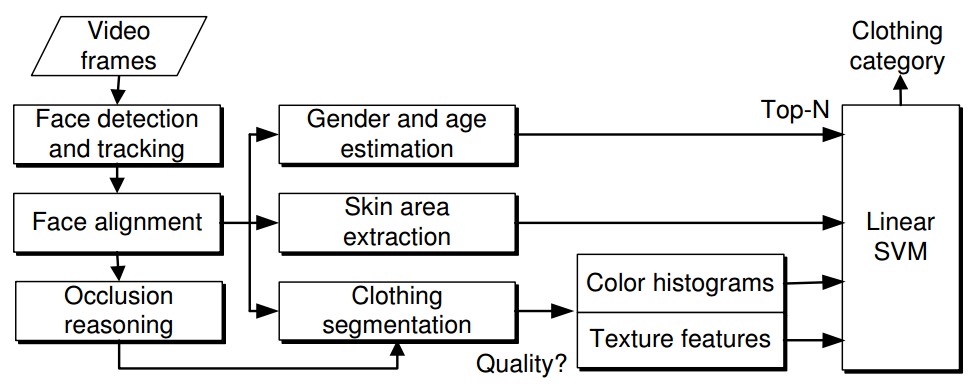
\includegraphics[scale=0.5]{images/Clothing_Diagram_1.png}
\caption{Video content analyses system diagram.}
\label{fig:vcasd}
\end{figure}
\FloatBarrier

A proper human figure alignment and clothing segmentation are required to
perform feature extraction and clothing classification. The results from
clothing segmentation might not be reliable for every frame. It is employed a
few cloth instances, with good segmentation quality, to calculate the average
feature vector to represent a cloth. A cloth is represented by ten instances,
including: gender and age estimation; skin ratio of arms and legs; 2D color
histograms; three texture descriptors.
\ac{HOG} is one of the used texture descriptors, to extract the features of
multiple spacial cells, drawn in figure ~\ref{fig:dtf}a ~\citep{1} as white
rectangles. The \ac{BoW}, another descriptor used, receives a bag of dense
\ac{SIFT} features, figure ~\ref{fig:dtf}b ~\citep{1}. The last texture descriptor
used is \ac{DCT}, figure ~\ref{fig:dtf}c ~\citep{1} In furtherance of better
results, clothes are analyzed in two sections, top and bottom, as represented
in figure ~\ref{fig:dtf} ~\citep{1}.

\begin{figure}[!h]
\centering
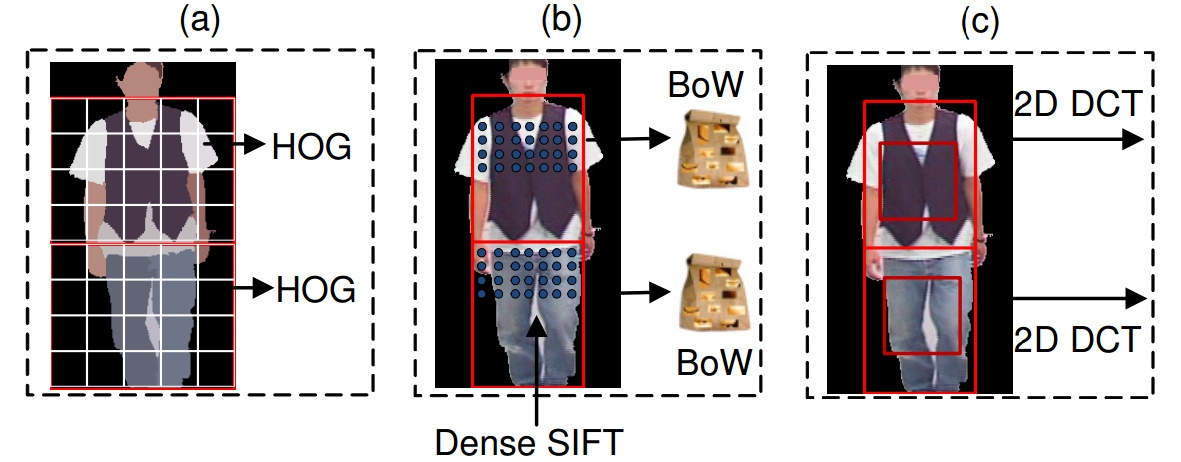
\includegraphics[scale=0.3]{images/top_bottom.jpg}
\caption{Different textures features based on \ac{HOG}, \ac{BoW} and
\acs{DCT} responses.}
\label{fig:dtf}
\end{figure}
\FloatBarrier

All the previously mentioned instances of a cloth are concatenated as the
clothing representation. Each clothing category is learnt by a
one-against-all linear \ac{SVM}.

The precision rate of the presented system goes from 45.0\% up to 90.3\%,
in short-pants and short-skirts respectively, as shown in table ~\ref{tab:prds}
 ~\citep{1}.

\begin{table}
\centering
\begin{tabular}{|l|r|}
\hline
\textbf{Category} & \textbf{Precision}\\
\hline
\hline
\textbf{Suit (top)} & 87.5\% \\
\hline
\textbf{Suit (bottom)} & 85.7\% \\
\hline
\textbf{Shirt} & 81.8\% \\
\hline
\textbf{T-shirt} & 70.7\% \\
\hline
\textbf{Jeans} & 90.1\% \\
\hline
\textbf{Short pant} & 45.0\% \\
\hline
\textbf{Short skirt} & 90.3\% \\
\hline
\textbf{Long skirt} & 74.7\% \\
\hline
\end{tabular}
\caption{Precision rate of the described system.}
\label{tab:prds}
\end{table}
\FloatBarrier

\section{Describing Clothing by Semantic Attributes}
\label{chap2:sec:art2}

The main focus of the system, described in \citep{2}, is dressing style
analysis. It is capable of, given a collection of photos, analysing the
dressing style, therefore, make shopping recommendations. An example is
represented in figure ~\ref{fig:ids}~\citep{2}. This is a fully automatic
system that learns attributes for clothing on the human upper body.

\begin{figure}[!h]
\centering
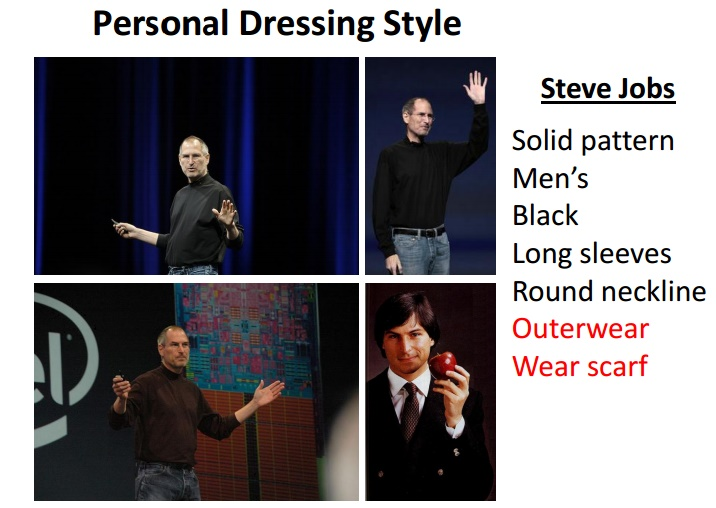
\includegraphics[scale=0.5]{images/2_3_fig0.jpg}
\caption{Inferred dressing style of a person. The wrong predictions are
highlighted in red.}
\label{fig:ids}
\end{figure}
\FloatBarrier

\begin{figure}[!h]
\centering
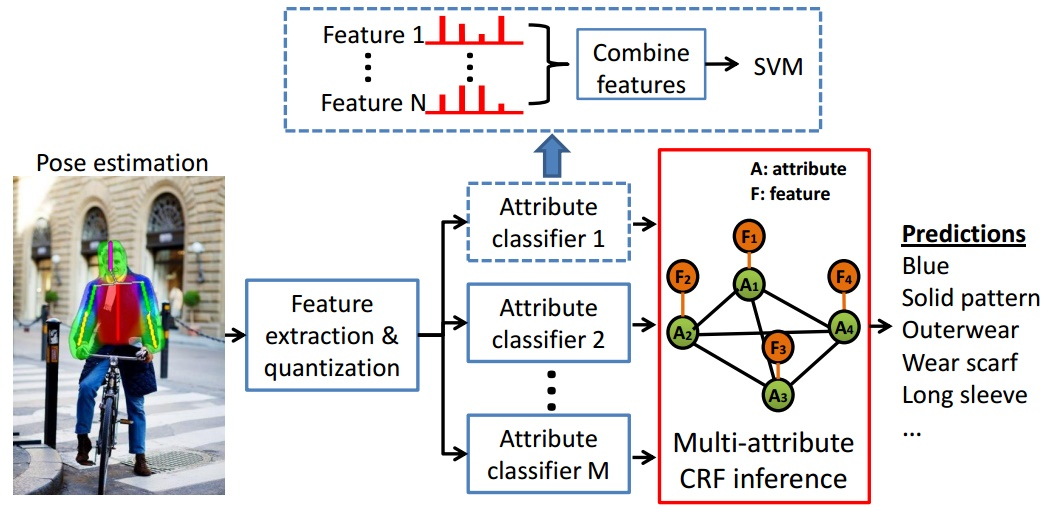
\includegraphics[scale=0.5]{images/2_3_fig2.jpg}
\caption{Flowchart of the system.}
\label{fig:fc}
\end{figure}
\FloatBarrier

In figure ~\ref{fig:fc}~\citep{2} is illustrated the flowchart of the presented
system. Since estimating full body pose is still a challenging problem, after
all, the lower body is not always visible or is sometimes occluded, so the
system only analyses the upper body. Given an input image, human
pose is estimated, finding the upper torso and arms location, as seen in the
example shown in figure ~\ref{fig:eehp}~\citep{2}. The upper body is detected
using a complementary upper body detector and a face detector. The person is
then segmented from the background using the GrabCut~\citep{7} algorithm.

\begin{figure}[!h]
\centering
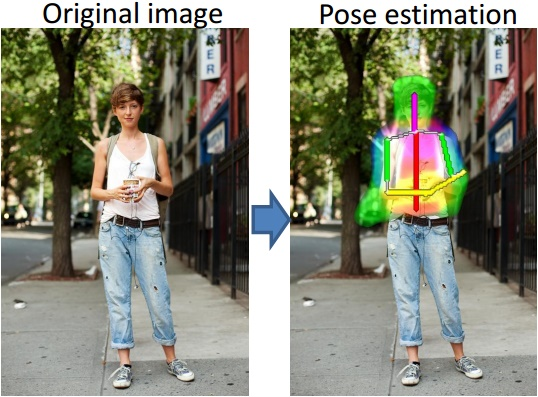
\includegraphics[scale=0.5]{images/2_3_fig1.jpg}
\caption{Example of the estimation of a human pose.}
\label{fig:eehp}
\end{figure}
\FloatBarrier

Following, forty features are extracted and quantized. Since the diversity of
clothing attributes desired to learn is wide, a single type of features is
not likely to be accurate on all of them. Accordingly, for each attribute, the
classification of several features are gathered to obtain a prediction. There
are four types of base features, extracted from: \ac{SIFT}; texture descriptors
from Maximum Response filters; color in LAB space; skin probabilities from skin
detector. The system takes advantage of the recent improvements in human pose
estimation, by adaptively extracting image features from different human body
parts. Therefore, the sampling location, scale and orientation of the \ac{SIFT}
descriptors depend on the estimation of the human pose. In figure ~\ref{fig:est}
~\citep{2}, it is represented the extraction of the \ac{SIFT} over the torso of
a person. The system, lastly, extracts one more feature, called skin-excluded
color feature. The skin area, generated by the skin detector, is masked out
to extract the skin-excluded color feature.

\begin{figure}[!h]
\centering
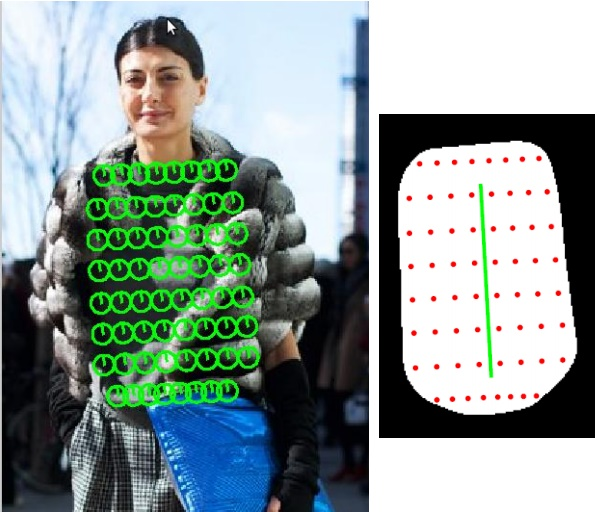
\includegraphics[scale=0.5]{images/2_3_fig3.jpg}
\caption{Extraction of the \ac{SIFT} over the torso region.}
\label{fig:est}
\end{figure}
\FloatBarrier

For each attribute, a \ac{SVM} classification is performed, using the
extracted traits. Each classifier produces a probability score.
Since clothing characteristics are correlated, mutual dependencies are also
explored between attributes. These dependencies then lead to the rules of style.
To the extent of modeling these rules, a \ac{CRF} is employed on top of the
classification provided by the individual classifiers. The inference result of
the \ac{CRF} produces the final list of attributes. Providing the probability
scores from the attribute classifier to the \ac{CRF}, leads to better results
than simply using a attribute classifier.

The precision rate of the presented system goes from 52.56\% up to 86.17\%,
in clothing attributes, as shown in table ~\ref{tab:ropsn}~\citep{2}. As for
clothing categories, rates go from 43.56\% to 80.65\%, ~\ref{tab:ropcc}
~\citep{2}.

\begin{table}
\centering
\begin{tabular}{|l|r|}
\hline
\textbf{Attribute} & \textbf{Accuracy}\\
\hline
\hline
\textbf{No sleeve} & 86.17\% \\
\hline
\textbf{Short sleeve} & 64.90\% \\
\hline
\textbf{Long sleeve} & 84.04\% \\
\hline
\end{tabular}
\quad
\begin{tabular}{|l|r|}
\hline
\textbf{Attribute} & \textbf{Accuracy}\\
\hline
\hline
\textbf{V-shape} & 67.27\% \\
\hline
\textbf{Round} & 52.56\% \\
\hline
\textbf{Other style} & 54.71\% \\
\hline
\end{tabular}
\caption{Rate of predictions referring to sleeve length (left table) and
neckline shape (right table).}
\label{tab:ropsn}
\end{table}
\FloatBarrier

\begin{table}
\centering
\begin{tabular}{|l|r|}
\hline
\textbf{Clothing} & \textbf{Accuracy}\\
\hline
\hline
\textbf{Shirt} & 43.56\% \\
\hline
\textbf{Sweater} & 54.84\% \\
\hline
\textbf{T-shirt} & 80.65\% \\
\hline
\textbf{Outerwear} & 61.30\% \\
\hline
\textbf{Suit} & 66.13\% \\
\hline
\textbf{Tank top} & 79.04\% \\
\hline
\textbf{Dress} & 56.45\% \\
\hline
\end{tabular}
\caption{Rate of predictions referring to clothing categories.}
\label{tab:ropcc}
\end{table}
\FloatBarrier

\section{Getting the Look: Clothing Recognition and Segmentation for Automatic
Products Suggestions in Everyday Photos}
\label{chap2:sec:art3}
\citep{3} presents a system capable of automatically suggest relevant clothing
products, when provided with a single image. Figure~\ref{fig:qisci}~\citep{3}
shows a real world image, the query image, on the left, and the clothing product
suggestions, on the right.

\begin{figure}[!h]
\centering
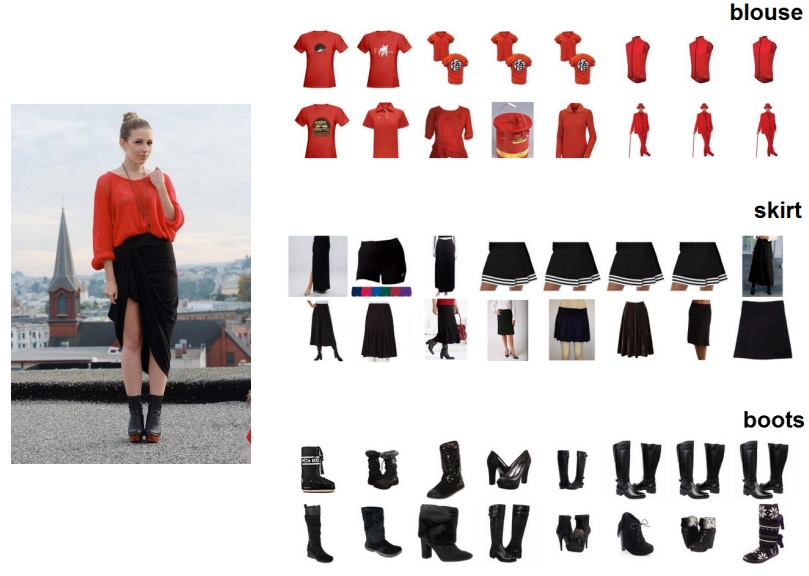
\includegraphics[scale=0.6]{images/2_4_fig1.jpg}
\caption{The query image and the suggested clothing items.}
\label{fig:qisci}
\end{figure}
\FloatBarrier

The direction chosen, in order to achieve the presented results, is divided in
two main courses: detecting the clothing classes represented in a given image
and obtaining visually alike products.

For the clothing classification, first is performed a pose estimation,
based on the pose estimation algorithm of~\citep{8}, explained in detail
in Section~\ref{chap3:sec:bps}. Once this step is complete, the main focus
turns to the image regions that are most likely to contain clothes.

Using the estimated pose areas, a prior probability map of clothing appearance
is calculated and then normalized on those regions. Given a set of classes,
firstly, a prior probability map is created for each clothing class.
Afterwards, the maps of all classes are concatenated and normalized,
creating a global \emph{clothing prior probability map}.
This probability map, subsequently, is used as a binary mask, so that only
probable human regions for clothing are used. In figure~\ref{fig:ppm}~\citep{3},
the probability maps for belt, feet, torso and hip regions (left) and
the global \emph{clothing prior probability map} (right).

\begin{figure}[!h]
\centering
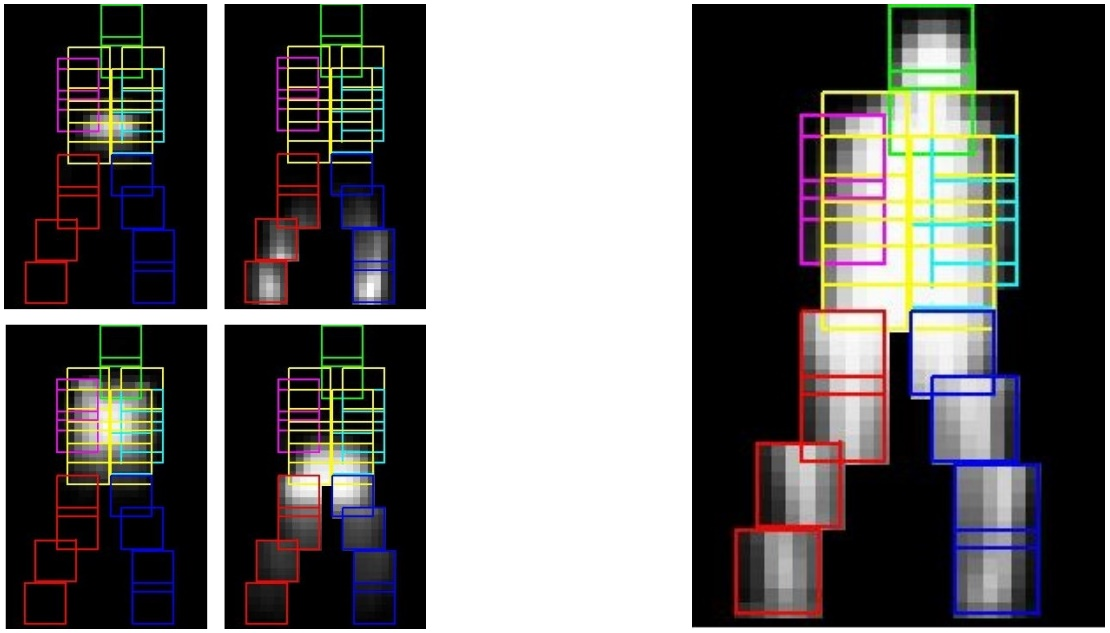
\includegraphics[scale=0.45]{images/2_4_fig2.jpg}
\caption{Prior probability maps, quantized and normalized, on estimated body
parts.}
\label{fig:ppm}
\end{figure}
\FloatBarrier

Once the aforesaid mask is calculated, it is possible to proceed to the
segmentation and clustering. In this phase, applying the binary mask, on the
detected body parts, is the primary step. This produces a image that only has
color in the regions of interest, as shown in the left image of figure
~\ref{fig:scs}~\citep{3}. Following, segmentation of \cite{9} is used, an
example of the results produced by it is presented in the middle image of
figure~\ref{fig:scs}~\citep{3}. Afterwards, to merge non-neighboring segments,
with the same visual appearance, a clustering step is performed on the extracted
segments. For the mentioned process, the adopted approach was the \ac{AGM}
algorithm~\citep{10}. In the right image of figure~\ref{fig:scs}~\citep{3}, are
the results of the merge between the clustering and the initial segments.


\begin{figure}[!h]
\centering
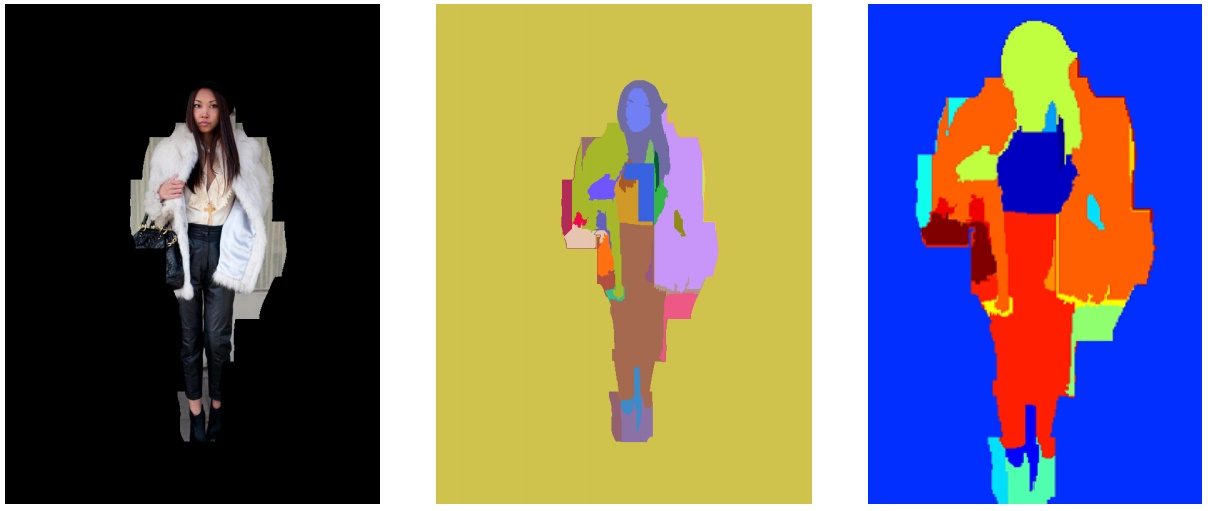
\includegraphics[scale=0.4]{images/2_4_fig3.jpg}
\caption{Segmentation and clustering steps.}
\label{fig:scs}
\end{figure}
\FloatBarrier

The next step consists on detecting if the segments correspond to a clothing
class and classify them. To accomplish this, four intuitions are considered: a
clothing class is always found in a consistent spacial region; clothing classes
are not distinguished solo by color and texture; shape alone is not enough
either, since there are highly inconsistent boundaries of clothing classes,
due to various human poses and views; representations must facilitate rapid
classification, therefore binary vectors are chosen to represent the segments.

Regarding the training set images, the exact clothing segment regions are given,
as well as their class label, making the process of segmentation and clustering
avoidable. Only the extraction of binary vectors is performed to each segment.
Matching each query vector with all training vectors is a poor choice in terms
of scalability. Accordingly, a sublinear algorithm is used to obtain the
most promising candidates. Once the binary vectors are extracted,
from each clothing segment of the training set, all the vectors of all segments
of all classes are added in a multi-probe \ac{LSH} index~\citep{11}, along
with the corresponding labels. Given a query vector, the \ac{LSH} index
returns the \emph{n} nearest neighbors of the query from the database, with
the corresponding classes. Subsequently, the probabilities, for each segment, are
calculated for each class, if it is higher than 0.5 the class is assigned to
that segment. Examples of this classification can be seen in figure
~\ref{fig:sccr}~\citep{3}.

\begin{figure}[!h]
\centering
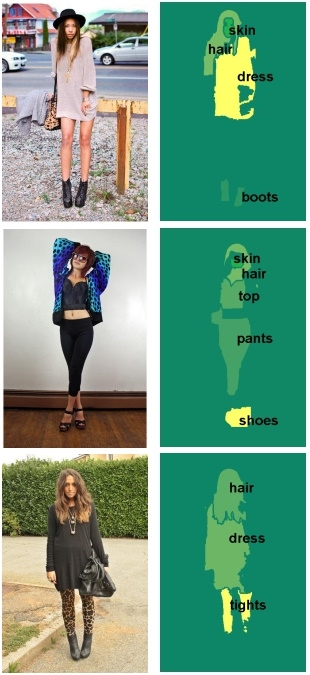
\includegraphics[scale=0.7]{images/2_4_fig4.jpg}
\caption{Sample of clothing classification results.}
\label{fig:sccr}
\end{figure}
\FloatBarrier

The next step consists in finding similar clothing suggestions from a large
product database. To segment the region of interest of the product in the
database, the GrabCut algorithm is used \citep{7}. Then to describe the visual
features of a region, color and texture characteristics are extracted.  After
having a characteristic vector for each image of the product collection, it is
necessary to retrieve the vectors that are similar to the query region vector.
The query vectors are classified, so it is only necessary to search for
familiar product within that class. To accomplish this, it is used a fast
approximate \ac{KNN} index, using a forest of \emph{randomized kd-trees}
~\citep{12}. For each search, the \emph{k} most similar products are selected
and then threshold the distance, so that only the closest results to the query
are displayed. If no results are below the distance threshold, that query
region is simple ignored.

\begin{table}
\centering
\begin{tabular}{|l|c|c|}
\hline
\textbf{Clothing Category} & \textbf{Relevant} & \textbf{Random}\\
\hline
\hline
\textbf{Dress} & 68\% & 10\% \\
\hline
\textbf{Skirt} & 59\% & 2\% \\
\hline
\textbf{Blouse} & 37\% & 4\% \\
\hline
\textbf{Top} & 55\% & 6\% \\
\hline
\textbf{Jackets \& Coats} & 43\% & 3\% \\
\hline
\textbf{Pants \& Jeans} & 69\% & 12\% \\
\hline
\textbf{Boots} & 66\% & 14\% \\
\hline
\hline
\textbf{All} & 54\% & 8\% \\
\hline
\end{tabular}
\caption{Evaluations of the suggested products.}
\label{tab:uesp}
\end{table}
\FloatBarrier

In order to test the developed system in large scale, a web application was
created. Provided with a real-world image, the application detects the clothing
classes existent, suggesting alike clothing products, for each class. Each
suggested product was evaluated as relevant, not relevant or random. The
results of the performed test are shown in table~\ref{tab:uesp}~\citep{3}.
Overall, the system suggested accurately 54\% of the products and had an
average of 8\% random suggestions.

\section{High-Level Clothes Description Based on Colour-Texture and Structural
Features}
\label{chap2:sec:art4}

\section{Mobile Visual Clothing Search}
\label{chap2:sec:art5}

\section{Conclusions}
\label{chap2:sec:concs}

\chapter{Implementation}
\label{chap:imp}

\section{Introduction}
\label{chap3:sec:intro}

\section{Background Subtraction}
\label{chap3:sec:bs}

\section{Body Pose Estimation}
\label{chap3:sec:bps}

\section{Color and Texture Extraction}
\label{chap3:sec:cte}

\section{Classification}
\label{chap3:sec:nnt}

\section{Conclusions}
\label{chap3:sec:concs}

\chapter{Tests and Results}
\label{chap:res}

\section{Introduction}
\label{chap4:sec:intro}

\section{}
\label{chap4:sec:...}

\section{Conclusions}
\label{chap4:sec:concs}

\chapter{Conclusions and Future Work}
\label{chap:cfw}

\section{Main Conclusions}
\label{sec:main-conc}

Esta secção contém a resposta à questão: \\
\emph{Quais foram as conclusões princípais a que o(a) aluno(a) chegou no fim
deste trabalho?}

\section{Future Work}
\label{sec:future-work}

Esta secção responde a questões como:\\
\emph{O que é que ficou por fazer, e porque?}\\
\emph{O que é que seria interessante fazer, mas não foi feito por não ser
exatamente o objetivo deste trabalho?}\\
\emph{Em que outros casos ou situações ou cenários -- que não foram estudados
no contexto deste projeto por não ser seu objetivo -- é que o trabalho aqui
descrito pode ter aplicações interessantes e porque?}

% SE EXISTIREM APENDICES, DESCOMENTAR O QUE ESTÁ EM BAIXO
% \appendix
% \include{apendice1}
% \clearpage{\pagestyle{empty}\cleardoublepage}
% \include{continuacao}
% \clearpage{\pagestyle{empty}\cleardoublepage}
% \include{apendice2}
% \clearpage{\pagestyle{empty}\cleardoublepage}
% \include{apendice3}
% \clearpage{\pagestyle{empty}\cleardoublepage}

\backmatter

\bibliographystyle{apalike-url}
\bibliography{bibliography}

\end{document}
